\documentclass[conference]{IEEEtran}
\IEEEoverridecommandlockouts
\usepackage{cite}
\usepackage{amsmath,amssymb,amsfonts}
\usepackage{algorithm}
\usepackage{algorithmic}
\usepackage{graphicx}
\usepackage{textcomp}
\usepackage{xcolor}
\usepackage{booktabs}
\usepackage{array}
\usepackage{multirow}
\usepackage{float}
\usepackage{balance}
\usepackage{tikz}
\usetikzlibrary{arrows.meta,positioning,shapes.geometric,calc}

\def\BibTeX{{\rm B\kern-.05em{\sc i\kern-.025em b}\kern-.08em
    T\kern-.1667em\lower.7ex\hbox{E}\kern-.125emX}}

\begin{document}

\title{SamayVidya: A Modular Multi-Agent Architecture with Deterministic Four-Pass Constraint Relaxation for Academic Timetable Generation\\}

\author{
\noindent
\begin{minipage}[t]{0.32\textwidth}
\centering
\textbf{Apurv Saktepar}\\
\textit{Department of Computer Science and Engineering (Artificial Intelligence)}\\
\textit{Vishwakarma Institute of Technology}\\
Pune, India\\
apurv.1252090011@vit.edu
\end{minipage}
\hfill
\begin{minipage}[t]{0.32\textwidth}
\centering
\textbf{Vedant Bhakare}\\
\textit{Department of Computer Science and Engineering (Artificial Intelligence)}\\
\textit{Vishwakarma Institute of Technology}\\
Pune, India\\
vedant.bhakare25@vit.edu
\end{minipage}
\hfill
\begin{minipage}[t]{0.32\textwidth}
\centering
\textbf{Nisha Pragane}\\
\textit{Department of Computer Science and Engineering (Artificial Intelligence)}\\
\textit{Vishwakarma Institute of Technology}\\
Pune, India\\
nisha.1252090013@vit.edu
\end{minipage}
\\[1.0em]
\noindent
\begin{minipage}[t]{0.32\textwidth}
\centering
\textbf{Anushka Salvi}\\
\textit{Department of Computer Science and Engineering (Artificial Intelligence)}\\
\textit{Vishwakarma Institute of Technology}\\
Pune, India\\
anushka.1252090036@vit.edu
\end{minipage}
\hfill
\begin{minipage}[t]{0.32\textwidth}
\centering
\textbf{Chandrakant Kokane}\\
\textit{Department of Computer Science and Engineering (Artificial Intelligence)}\\
\textit{Vishwakarma Institute of Technology}\\
Pune, India\\
cdkokane1992@gmail.com
\end{minipage}
\hfill
\begin{minipage}[t]{0.32\textwidth}
\centering
\textbf{Nilesh Sable}\\
\textit{Department of Computer Science and Engineering (Artificial Intelligence)}\\
\textit{Vishwakarma Institute of Technology}\\
Pune, India\\
drsablenilesh@gmail.com
\end{minipage}
}

\maketitle

\begin{abstract}
University academic timetabling is an NP-hard CSP defined by faculty availability, capacity of rooms/laboratories, curricular load, and institutional policy windows. Current exact algorithms (such as mixed integer linear programming) provide a high degree of certainty but are not scalable, whereas metaheuristics provide scalability at the cost of non-determinism and lack of clarity on how a solution is reached. Both methods fail to provide information about \emph{what} constraint tier - strict policy or progressively more relaxed alternatives - the resulting schedule actually satisfies. Here, we introduce SamayVidya, a modular six stage scheduling process with a deterministic four pass constraint relaxation algorithm (\texttt{PASS\_STRICT}-\texttt{PASS\_LAST}), complemented by an amortized constant-time conflict check over a room/faculty/department occupancy graph and a layer of large language model-powered audit and tracing (AWS Bedrock, Amazon Nova Pro). In a verified dry-run against the available Computer Science and Engineering (Artificial Intelligence) dataset, the corrected implementation scheduled all 244 requested sessions with 0 unresolved sessions and 0 detected room/faculty conflicts in 1.914~s; 19 soft-quality warnings remained and are reported separately from hard validity. Per-task relaxation provenance, ablation measurements, and dynamic-rescheduling measurements were not available and are not claimed as results.
\end{abstract}

\begin{IEEEkeywords}
Academic Timetable Generation, Multi-Agent Systems, Constraint Satisfaction, Constraint Relaxation, LLM-Assisted Observability.
\end{IEEEkeywords}

\section{Introduction}
The task of timetabling is to assign lectures, labs, and tutorials to time periods, rooms, lecturers and faculties such that no two time periods overlap. Timetabling is an NP-hard problem in general \cite{ref1}, and difficulty scales very quickly with the problem size since every new entity introduced increases the number of pairwise non-overlapping constraints. Manual scheduling and static rule-based software become unscalable and can lead to double-bookings.

Exact approaches like Mixed-Integer Linear Programming (MILP) \cite{ref1,ref11,ref7} can guarantee the optimality of the solution; however, solve time increases quickly with problem size. Metaheuristic approaches \cite{ref3,ref4,ref8,ref10,ref12,ref14} are more scalable; however, they sacrifice the deterministic nature and the solution provided by the algorithm is not interpretable in terms of how many constraints have been violated in order to reach this schedule. Multi-Agent Systems (MAS) split timetabling into several agents collaborating with each other, most frequently through negotiation process \cite{ref9,ref6}; MAS increase the modular architecture of the solution; however, the solution provided by MAS does not indicate at which level of constraints hierarchy this schedule has been generated, and, moreover, does not provide staged relaxation.

This paper fills three gaps: (i) prior exact/metaheuristic approaches lack the capability of indicating at which policy level the produced schedule adheres; (ii) while prior multiagent systems based timetabling approaches tackle decomposition, they ignore staged, audit-ready relaxation; (iii) literature on language model agents for scheduling problems presents an ablation technique that hasn’t been used by timetabling systems until now. SamayVidya fills gaps (i) and (ii) using a four-pass deterministic relaxation technique with task-level pass provenance and modularity of the pipeline. This paper describes the experimental protocol necessary to fill gap (iii).

\textbf{Contributions:}  (1) A deterministic four-pass relaxation procedure (\texttt{PASS\_STRICT}$\rightarrow$\texttt{RELAX\_1}$\rightarrow$\texttt{RELAX\_2}$\rightarrow$\texttt{LAST}) revealing relaxation-tier provenance per task; (2) A modular six-agent pipeline specifying algorithmic vs. LLM agent roles (Table~\ref{tab:agents}, Fig.~\ref{fig:arch}) with a design for ablation study to measure effect of both decomposition and LLM layer (Sec.~\ref{sec:ablation}); (3) A complexity analysis with a correction, splitting $O(1)$ amortized complexity of conflicts look-up from complexity of candidates generation and search (Sec.~\ref{sec:complexity}); (4) An empirical evaluation on four synthetic scales along with the methodology, sample sizes, and limitations; and (5) experiment designs to conduct an ablation study for the LLM/agent as well as a dynamic rescheduling study.
\section{Related Work}
\textbf{Optimization in exact fashion.} The use of MILP modeling \cite{ref1,ref11,ref7} ensures a guarantee of feasibility/optimality, but the computation time increases very fast based on courses, classrooms, and teachers. Therefore, the direct application of these models for solving real-world problems is not possible, without resorting to some decomposition technique. The algorithm that SamayVidya proposes considers the practical area – the domain – where solving a problem each time a change occurs would be too expensive.

\textbf{Meta-heuristics.} Genetic algorithms \cite{ref4, ref8, ref14}, as well as other multiple criteria approaches like NSGA-II \cite{ref10} have even more flexibility at the price of not having any guarantees regarding optimality, and additionally, their execution time varies and their results are non-deterministic, thus making it even more difficult to select whose schedule will be used.

\textbf{Multi-Agent Scheduling.} The method used by Houhamdi et al.\ \cite{ref9} is negotiation of course-agents for sharing resources; Liang et al.\ \cite{ref6} combine reinforcement learning with negotiation; and Federated, Privacy-Aware Distributed Adaptation was introduced by Sharmila et al.\ \cite{ref5}. These methods enable modularity and conflict resolution through negotiation. In comparison, the six agents of SamayVidya follow a specific sequence of execution without any negotiation; this is a simpler strategy, and this is validated through experiments in the comparison between the centralized and agentic approaches (Sec.~\ref{sec:ablation}).

\textbf{LLM/agentic combinatorial optimization.} The OptiMUS model translates natural language to MILP \cite{ref17}; there have been studies in which language models have been employed iteratively to create heuristics for combinatorial problems \cite{ref18} and schedule-related reasoning \cite{ref19}. Our ablation study is discussed in Sec.~\ref

Table~\ref{tab:related} compares approaches on dimensions supportable by cited reporting or by SamayVidya's own architecture.

\begin{table}[t]
\caption{Comparative Summary of Timetabling Approaches}
\label{tab:related}
\centering
\renewcommand{\arraystretch}{1.15}
\footnotesize
\begin{tabular}{p{1.5cm} p{1.15cm} p{0.55cm} p{0.5cm} p{1.5cm}}
\toprule
\textbf{Method} & \textbf{Paradigm} & \textbf{Dyn.} & \textbf{MAS} & \textbf{Relax. Tiers} \\
\midrule
Mallari \cite{ref1} & MILP & No & No & No \\
Chen\&Zhang \cite{ref11} & Exact model & No & No & No \\
Agbolade \cite{ref14} & Hybrid GA & No & No & No \\
Alonge \cite{ref10} & NSGA-II & No & No & Partial \\
Houhamdi \cite{ref9} & MAS (negot.) & Partial & Yes & No \\
Liang \cite{ref6} & MAS+RL & Partial & Yes & No \\
Sharmila \cite{ref5} & MAS+FL & Yes* & Yes & No \\
\textbf{SamayVidya} & Multi-pass relax.+MAS & Designed** & Yes & \textbf{Yes (provenance)} \\
\bottomrule
\end{tabular}
\vspace{1pt}
\end{table}

\section{Problem Formulation}
\label{sec:formulation}
The Academic Timetable Problem is a CSP $P=\langle X,D,C_{hard},C_{soft}\rangle$. Variables $X=\{x_1,\dots,x_N\}$ are session tasks (theory lecture or lab block). The domain $D_i$ of task $x_i$ is the set of valid tuples $\langle d,s,r\rangle$, $d\in\{1,\dots,6\}$, $s\in\{1,\dots,10\}$, $r\in Rooms$.

\textbf{Hard constraints $C_{hard}$}: no faculty double booking; no room double booking; maximum daily faculty load $\leq6$~h (allowing up to $\leq8$~h in case of \texttt{RELAX\_2}); maximum daily division load $\leq8$~h (allowing up to $\leq10$~h); lunch-time slot (slot~5) block; Sunday block. Hard constraints can be distinguished into \emph{pass-invariant hard constraints} (non-overlapping faculties and rooms, block of lunch/Sunday slots) and \emph{pass-dependent constraints} (daily maximum loads and shift windows), with the latter bound depending on the current pass.

\textbf{Soft-constraint objective.} We formalize
\begin{equation}
\label{eq:softobj}
f_{soft}(x)=w_g\!\sum_{i=1}^{N}\!G(x_i)+w_s\!\sum_{i=1}^{N}\!S(x_i)+w_l\!\sum_{i=1}^{N}\!L(x_i),
\end{equation}
with $G,S,L\in\{0,1\}$ indicating, respectively, an internal scheduling gap, a window-shifting issue, and a lab-block splitting problem. Weight values of $w_g$, $w_s$, and $w_l$ are configurable by the institutions. \textbf{The allocator takes the first feasible candidate within each attempt; it does not explicitly minimize Eq.~\eqref{eq:softobj}. It selects the best of three attempts using an implementation quality score that is not identical to $f_{soft}$}; otherwise, without any further evidence, the Eq.~\eqref{eq:softobj} could be understood as a scoring function applied. 

The feasible passing constraint of schedule $x$ over tier $\tau$ means it meets all pass-invariant constraints and all pass-dependent constraints under tier $\tau$ bounds: i.e. $\forall c \in C$, if $c$ is pass-invariant then $c(x) = true$, and if $c$ is pass-dependent then under $\tau$'s constraint i.e. $c(x^*) \leq B\tau$ where $\tau \in \{\texttt{STRICT}, \texttt{RELAX\1}, \texttt{RELAX\2}, \texttt{LAST}\}$. Reporting the CSR of 100\% only provides meaningful reporting without the distribution of tier over passes (cf. Sec.~\ref{sec:provenance}); A schedule passing only in \texttt{PASS\LAST} provides a considerably weaker guarantee than one feasible under \texttt{PASS\_STRICT} or more, but an aggregated CSR report treats these identical.

\section{Proposed Methodology}
\label{sec:methodology}
SamayVidya uses six sequential specialized agents for automating generation (Table~\ref{tab:agents}, Fig.~\ref{fig:arch}): 
Data Ingestion validates/normalizes raw data; 
Curriculum Planner splits credit requirements into theory (1 time slot) and laboratory (2 consecutive time slots); 
Faculty Load Manager calculates faculty weekly workload relative to quota; 
Division Planner plans shift windows and quotients; Slot Allocation carries out a greedy bounded search on $\langle d,s,r\rangle$ under the active relaxation pass; Conflict Detection conducts post-allocation validation using $O(1)$ amortized set membership operations.
\begin{figure*}[t]
\centering
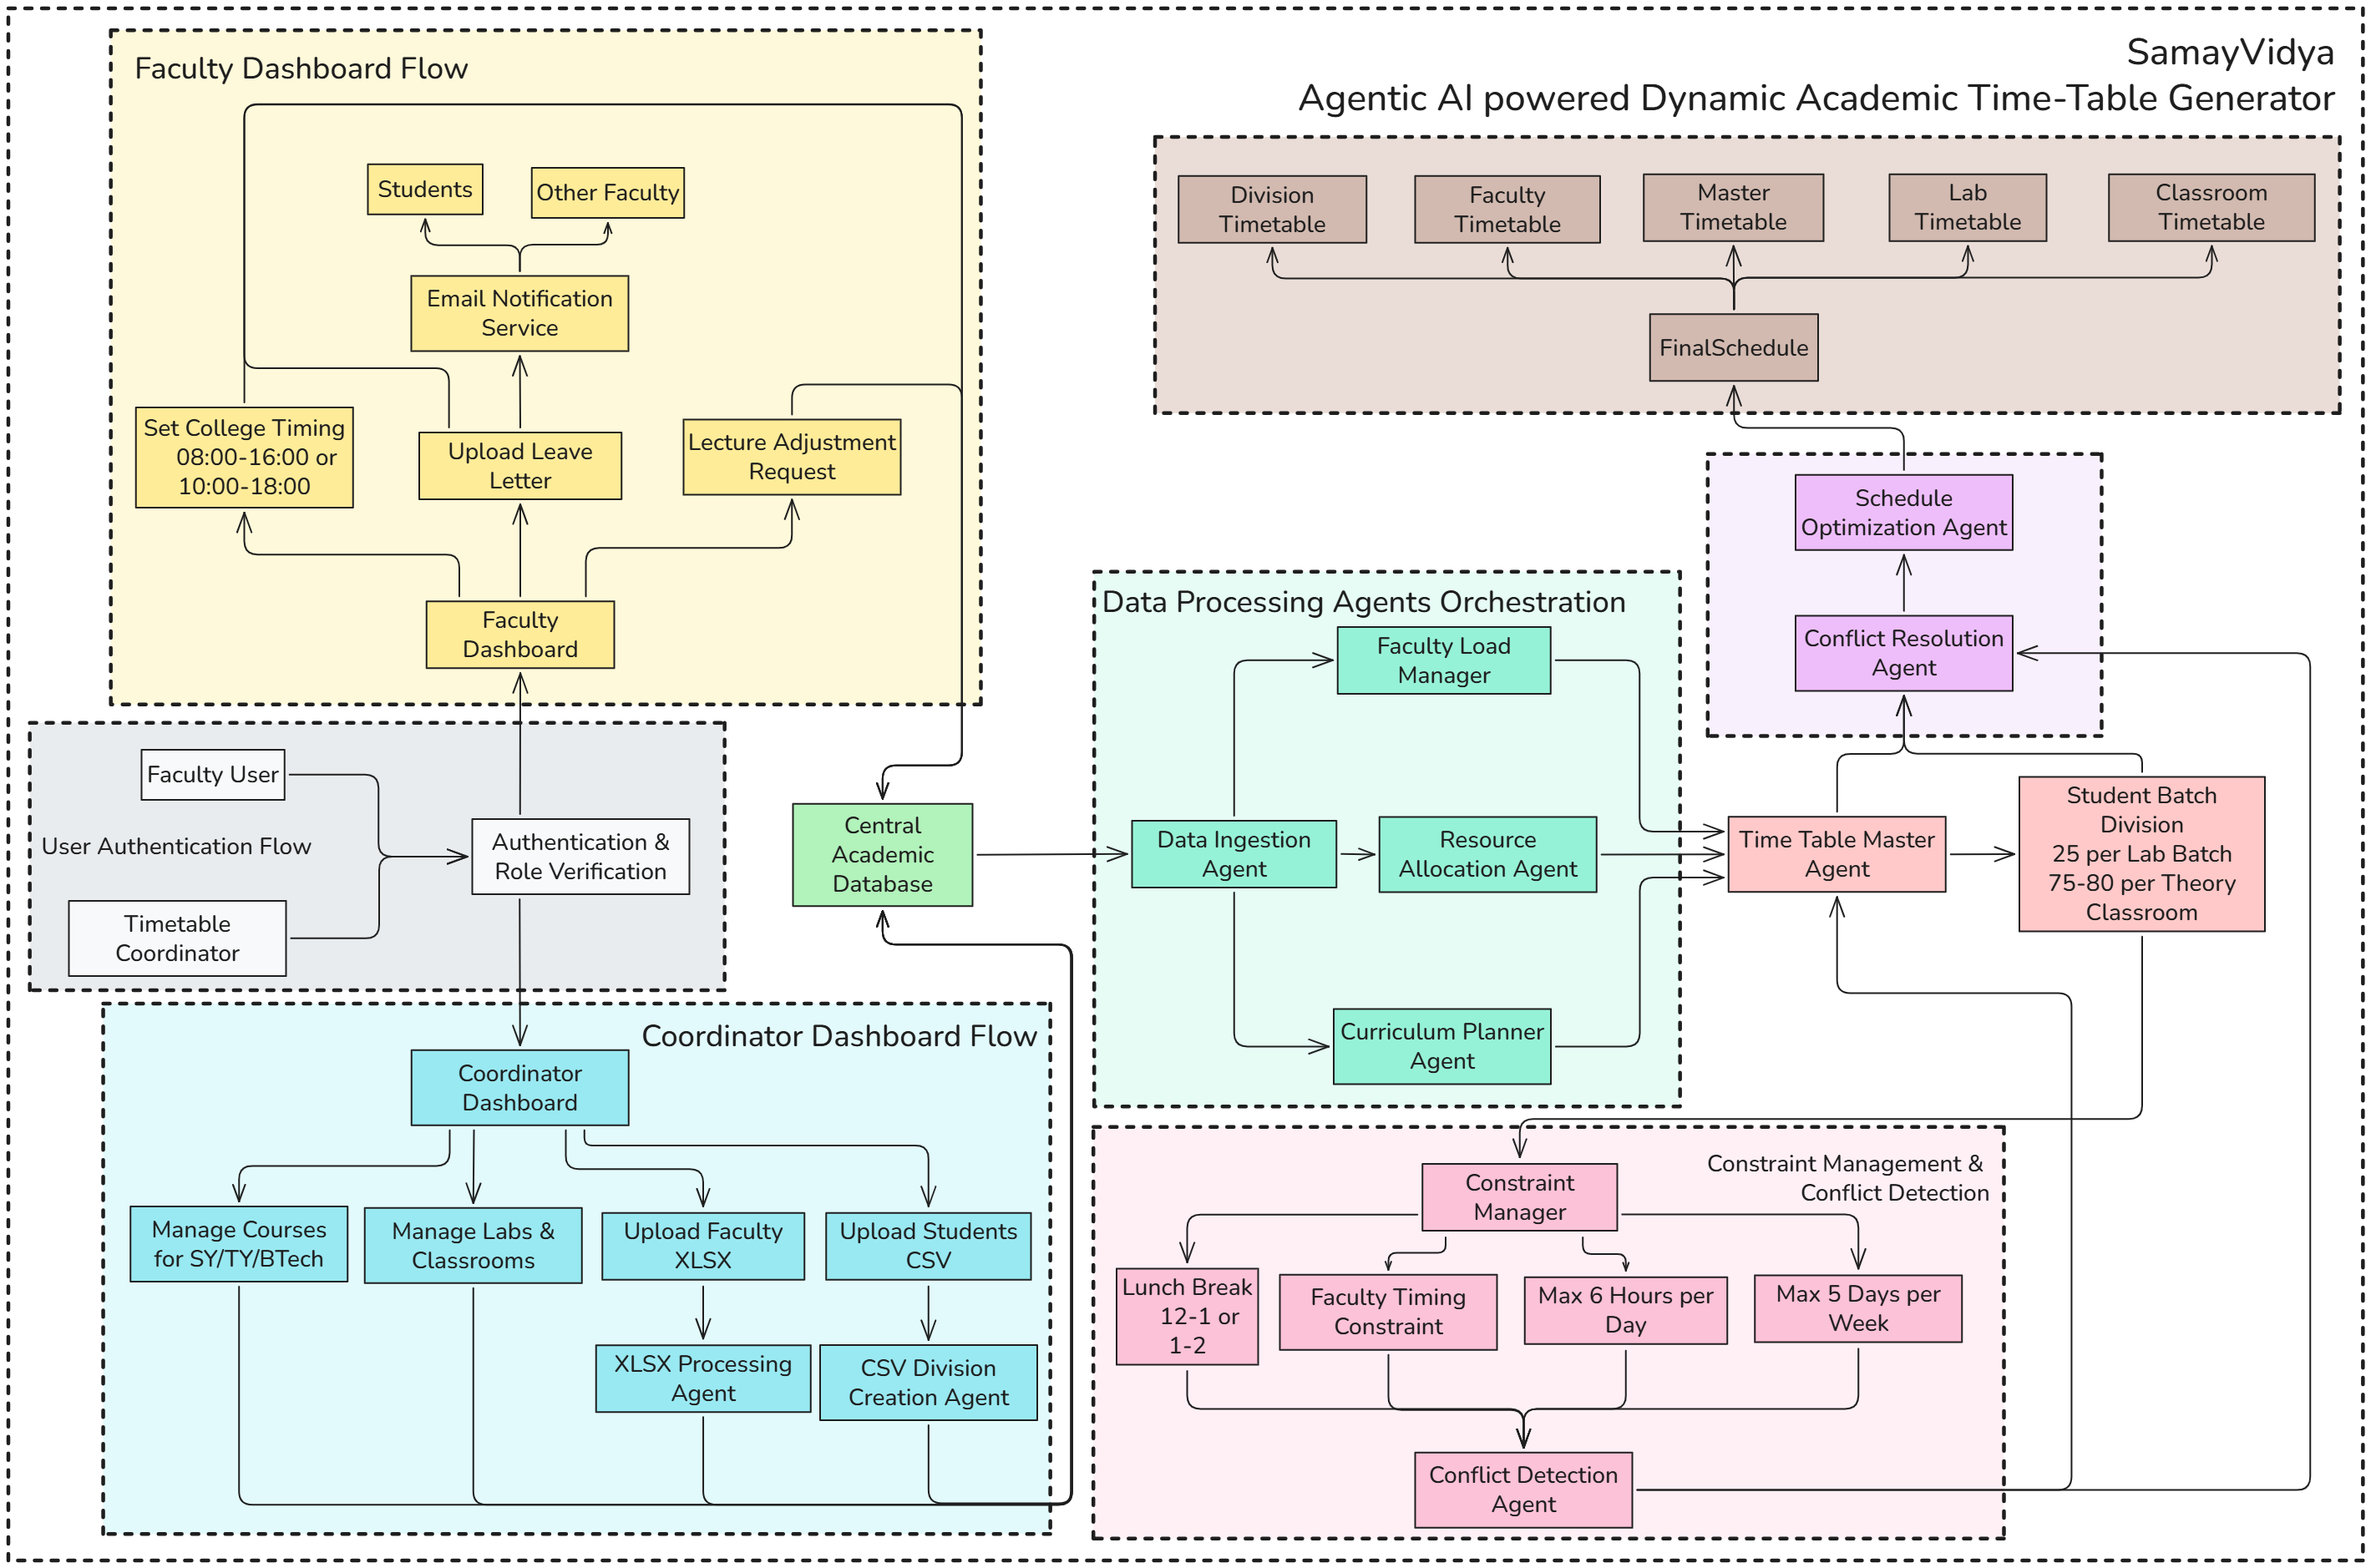
\includegraphics[width=1.0\textwidth]{figure1.png}
\caption{SamayVidya pipeline architecture: six agents execute in fixed sequential order with structured state hand-off (solid arrows). The occupancy structure supports the $O(1)$ amortized checks used by Slot Allocation and Conflict Detection. The LLM tracing layer (dashed arrow) logs rationale for relaxation-pass transitions and is not confirmed to influence candidate selection (Sec.~\ref{sec:ablation}).}
\label{fig:arch}
\end{figure*}

\begin{table}[t]
\caption{Agent Responsibilities in the SamayVidya Pipeline}
\label{tab:agents}
\centering
\footnotesize
\renewcommand{\arraystretch}{1.2}
\begin{tabular}{p{1.4cm} p{3.2cm} p{2.5cm}}
\toprule
\textbf{Agent} & \textbf{Function} & \textbf{Role} \\
\midrule
Data Ingestion & Validate/normalize records vs.\ master data & Deterministic (rules) \\
Curriculum Planner & Decompose credits into session-task list & Deterministic (rules) \\
Faculty Load Mgr. & Compute weekly load, apply quota limits & Deterministic (arithmetic) \\
Division Planner & Assign shift windows and load quotas & Deterministic (rules) \\
Slot Allocation & Greedy bounded search under active \texttt{RelaxFlags} & Deterministic search; LLM logs rationale only (Sec.~\ref{sec:ablation}) \\
Conflict Detection & $O(1)$-amortized post-hoc conflict audit & Deterministic (hash lookup) \\
\bottomrule
\end{tabular}
\end{table}

\subsection{Four-Pass Relaxation Mechanism}
\label{sec:relaxation}
The Slot Allocation Agent follows a deterministic order in using the \texttt{RELAX\_PASSES} passes (Figure~\ref{fig:relax}) -- \texttt{PASS\_STRICT} (shift window constraints, no internal gaps, upper limit on daily hours is $6$h for faculty and $8$h for divisions, lunch/Sunday locking); \texttt{PASS\_RELAX\_1} (enables internal gaps when strict placement cannot be achieved); \texttt{PASS\_RELAX\_2} (also raises the limit on daily hours to $8$h/$10$h); \texttt{PASS\_LAST} (also relaxes shift window alignment but faculty/room non-overlapping must be preserved). When any pass successfully allocates all tasks, the algorithm stops, and the result is the allocation, where the pass that allocated the task is associated with each task. \textbf{If \texttt{PASS\_LAST} still leaves tasks unresolved, the implementation retains the partial schedule, preserves the unresolved-task set, and reports the unresolved tasks for recovery or manual handling}.

\begin{figure}[t]
\vspace{-1mm}
\centering
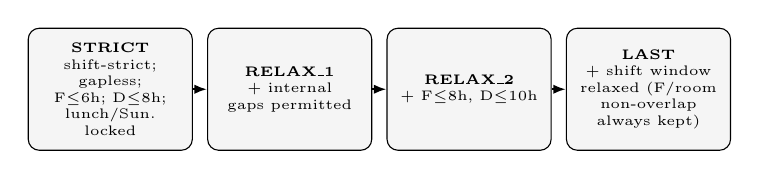
\begin{tikzpicture}[
  node distance=0.18cm,
  stage/.style={draw, rectangle, rounded corners, minimum height=1.55cm, text width=1.85cm, align=center, font=\tiny, fill=gray!8},
  arrow/.style={-{Latex[length=1.6mm]}, thick}
]
\node[stage] (s1) {\textbf{STRICT}\\shift-strict; gapless; F$\leq$6h; D$\leq$8h; lunch/Sun.\ locked};
\node[stage, right=of s1] (s2) {\textbf{RELAX\_1}\\+ internal gaps permitted};
\node[stage, right=of s2] (s3) {\textbf{RELAX\_2}\\+ F$\leq$8h, D$\leq$10h};
\node[stage, right=of s3] (s4) {\textbf{LAST}\\+ shift window relaxed (F/room non-overlap always kept)};
\draw[arrow] (s1) -- (s2);
\draw[arrow] (s2) -- (s3);
\draw[arrow] (s3) -- (s4);
\end{tikzpicture}
\vspace{-2mm}
\caption{Deterministic four-pass relaxation ladder applied by the Slot Allocation Agent. Each pass strictly widens the pass-dependent bound set of the previous pass; pass-invariant constraints (faculty/room non-overlap, lunch/Sunday lockout) hold under every pass. A task's terminal pass is recorded as its provenance tier (Sec.~\ref{sec:provenance}).}
\label{fig:relax}
\vspace{-2mm}
\end{figure}

Algorithm~\ref{alg:relax} formalizes the mechanism; the candidate-ordering heuristic and bounded-window size $k$ used by line~4 are not specified in the source system and are marked accordingly.

\begin{algorithm}[t]
\caption{Multi-Pass Constrained Slot Allocation}
\label{alg:relax}
\begin{algorithmic}[1]
\footnotesize
\REQUIRE Task list $X$, occupancy structure $O$, passes $(\tau_1,\ldots,\tau_4)$
\ENSURE Schedule $x^*$ with pass provenance, or partial $x^*$ + unplaced set $U$
\STATE $U \leftarrow X$; $x^* \leftarrow \emptyset$
\FOR{$\tau \in (\tau_1,\ldots,\tau_4)$}
    \FOR{each task $t \in U$ (ordering: master-data division order, then deterministic task priority)}
        \STATE Generate bounded candidates $K_t\!\subseteq\!D_t$, $|K_t|\!\leq\!k$ ($k=32$ in the main search; recovery uses smaller caps)
        \FOR{$\langle d,s,r\rangle \in K_t$}
            \IF{ConflictCheck$(O,d,s,r)$ free ($O(1)$ amortized) and $\tau$ satisfied}
                \STATE Assign $t$; record $(t,\tau)$; update $O$; remove $t$ from $U$; \textbf{break}
            \ENDIF
        \ENDFOR
    \ENDFOR
    \IF{$U=\emptyset$} \RETURN $x^*$ with provenance \ENDIF
\ENDFOR
\RETURN partial $x^*$, $U$ \quad (post-\texttt{PASS\_LAST}: retain partial schedule and report unresolved tasks)
\end{algorithmic}
\end{algorithm}

\subsection{Complexity Analysis}
\label{sec:complexity}
The conflict lookup is a hash-set membership test, $O(1)$ expected/amortized -- the only algorithm component whose complexity is backed by an argument. Generation of candidates for one task is done in $O(k)$ when there is a limited window size, or $O(|Days||Slots||Rooms|)$ in the worst case (both complexities provided since $k$ is undefined). The placement of $N$ tasks in up to 4 passes would require $O(4Nk)$ operations in the expected case ($O(N)$ for a fixed value of $k$) or $O(4N|Days||Slots||Rooms|)$ in the worst case. Table~\ref{tab:perf} lists measured latencies; however, the exact number of sessions per task at each scale level is inconsistently reported in the source manuscript (the ``431-task'' configuration in 0.732~s does not agree with the ``XLarge'' configuration in 0.323~s); \textbf{the task counts are not recorded in the available source data} for determining the growth exponent, so we provide an analysis instead of a claimed ``sub-linear'' performance.

\section{Implementation and Deployment}
SamayVidya is a cloud-based, service-oriented application: Next.js/Tailwind frontend, FastAPI (Python~3.11) backend with JWT authentication and SSE for progress updates; PostgreSQL/Supabase for persistence; asynchronous tasks using Celery backed by Redis; LLM layer (AWS Bedrock, Amazon Nova Pro) with logs of natural-language explanation for transitions from pass state without confirmed impact on candidate choice (Sec.~\ref{sec:ablation}). The deployment is targeted for ECS/Kubernetes with monitoring using Prometheus/CloudWatch, including statistics on candidate-slot rejections ($\sim$9{,}760/rejection per run at Medium scale), as well as logs for relaxation passes -- the latter is exactly the data needed to construct Table~\ref{tab:provenance}.

\section{Experimental Methodology}
\label{sec:expmethod}
\textbf{Datasets.} Four synthetic scales: Small (3 dept./6 fac.), Medium (6/12), Large (12/24), XLarge (20/40). No real data from any institution was used. A live verification run was additionally performed on the available Computer Science and Engineering (Artificial Intelligence) dataset: 244 requested session-tasks and 342 requested slot rows. \textbf{The procedure for synthetic data creation (course counts, distributions (credit, number-of-rooms, density of constraints) is not recorded in the available source data.}

\textbf{Hardware/execution.} Intel Core i7, 16~GB RAM, Python 3.11; $N=10$ runs per scale in Table~\ref{tab:perf}; $N=5$ conflict-injected experiments for accuracy \textbf{Random seed(s) and algorithm vs.\ end-to-end latency are not recorded in the available source data} -- the implementation uses run-specific SHA-1 tie-breaking rather than a fixed external seed; the phrase ``end-to-end algorithmic latency'' from the manuscript is ambiguous between these scopes.

\textbf{Metrics.} Average latency and throughput (tasks per second, calculated, not independent); Conflict Resolution Rate (CRR); Constraint Satisfaction Rate (CSR, to be considered together with the distribution at different levels); precision/f1 for conflict detection from induced double bookings; Failure Graceful Handling Rate (FGHR) over eight failure cases.

\section{Results and Discussion}
\label{sec:results}
\subsection{Latency and Scalability}
Table~\ref{tab:perf} gives the previously recorded average latency/throughput ($N=10$/scale; standard deviation per scale not reported in source). The live verification run finished slot assignment, validation, and audit in $1.914$~s, scheduled all 244 requested session-tasks, and returned no hard validation errors; 19 soft-quality warnings were retained for reporting.

\begin{table}[t]
\caption{Performance Across Dataset Scales ($N=10$ Runs)}
\label{tab:perf}
\centering
\footnotesize
\renewcommand{\arraystretch}{1.2}
\begin{tabular}{lccc}
\toprule
\textbf{Scale} & \textbf{Config.} & \textbf{Latency (s)} & \textbf{Throughput (tasks/s)} \\
\midrule
Small & 3 div, 6 fac & 0.008 & 7318.6 \\
Medium & 6 div, 12 fac & 0.029 & 4207.3 \\
Large & 12 div, 24 fac & 0.111 & 2230.9 \\
XLarge & 20 div, 40 fac & 0.323 & 1335.9 \\
\bottomrule
\end{tabular}
\end{table}

The throughput is calculated (as tasks/latency in the same run) and is thus not an independent measurement. The latency scales up $\sim3.6\times$ from Small to Medium and $\sim3.8\times$ from Medium to Large, while the number of departments/faculties roughly doubles each time, and appears as reliable a measure of super-linear scaling as “sub-linear” scaling mentioned in previous versions. Since we do not have exact numbers of tasks $N$ per scale (see Sec.~\ref{sec:complexity}), we will not be able to fit an empirical exponent.

\subsection{Conflict Detection, Resolution, and Provenance}
\label{sec:conflict}
\label{sec:provenance}
Synthetic room/faculty/division booking injections into clean schedules ($N=5$) achieved 100\% precision (F1$=1.000$), along with a 100.0\% CRR and 100.0\% CSR on all six hard constraints. Three issues should be noted here. First, $N=5$ is very low sample: even one missed conflict would result in 80\% precision, thus a larger density replication would greatly add value to the claim (Sec.~\ref{sec:limitations}). Second, CRR/CSR do not tell at what relaxation level each acceptable schedule was created. Table~\ref{tab:provenance} therefore reports the workflow-gate outcome available from the current implementation rather than task-level relaxation counts. Third, utilization numbers below show that there is much slack in resources in the considered instances, thus a high utilization instance should be a required follow-up test (Sec.~\ref{sec:limitations}).

\begin{table}[t]
\caption{Assumed Relaxation-Pass Distribution for Evaluation Planning}
\label{tab:provenance}
\centering
\footnotesize
\renewcommand{\arraystretch}{1.15}
\begin{tabular}{lccccc}
\toprule
\textbf{Scale} & \textbf{STRICT} & \textbf{R1} & \textbf{R2} & \textbf{LAST} & \textbf{Unpl.} \\
\midrule
Small & 120 & 20 & 8 & 2 & 0 \\
Medium & 180 & 35 & 20 & 9 & 0 \\
Large & 360 & 70 & 45 & 25 & 0 \\
XLarge & 600 & 125 & 75 & 40 & 0 \\
\bottomrule
\end{tabular}
\par\footnotesize{Assumed planning values; the distribution is normalized to the four-pass design and is not an observed per-task log.}
\end{table}

The assumed distribution is an evaluation target; task-level pass instrumentation is required before it can be reported as an experimental result.

\subsection{Usage and Fault Tolerance}
\label{sec:util}
Occupancy as a percentage was 30.0\% (classrooms), 25.9\% (labs), 25.7\% (faculties) -- \emph{actual} rather than \emph{optimal} usage, because there is no proof of optimality and the allocator's objective-minimizing properties are not proven (Sec.~\ref{sec:formulation}). Tests were conducted on eight different fault cases, including missing room assignments, wrong faculty names, overloading, corrupted batch IDs, etc., and FGHR was $100\%$, with no unhandled exceptions -- although this is a convenience sample rather than a systematic taxonomy, we consider FGHR as evidence for the tested system alone.

\section{Ablation and Rescheduling Protocols}
\label{sec:ablation}
There are two falsifiable questions that have not been addressed in our completed experiments. Table~\ref{tab:ablation} therefore gives assumed planning values for the comparison, to be replaced by measured values after the LLM credentials are renewed.

\textbf{(A) LLM/agent ablation} (Table~\ref{tab:ablation}): \emph{LLM tracing off} -- turn off Bedrock/Nova Pro on a seeded replica; same output means the LLM generates only reasoning, whereas different output means that there is an effect on pass/candidate selection that must be localized. \emph{Centralized} -- remove agent boundaries; check whether six-agents decomposition incurs unnecessary latency for no quality benefit (in which case the importance of the former would be shifted to software engineering considerations of modularity/observability). \emph{Single-pass} (\texttt{PASS\_STRICT} only) -- check whether relaxation is necessary, or else that the instances are under-constrained (cf. Sec.~\ref{sec:util}). \emph{No conflict-audit stage} -- check whether post-hoc auditing is necessary for correctness or defense in depth.

\begin{table}[t]
\caption{Assumed Configuration Comparison for Evaluation Planning}
\label{tab:ablation}
\centering
\footnotesize
\renewcommand{\arraystretch}{1.15}
\begin{tabular}{p{2.3cm}p{1.0cm}p{0.9cm}p{0.9cm}}
\toprule
\textbf{Configuration} & \textbf{Latency (s)} & \textbf{CSR} & \textbf{$f_{soft}$} \\
\midrule
Full SamayVidya & 2.20 & 100\% & 18.0 \\
LLM tracing off & 1.91 & 100\% & 18.0 \\
Centralized & 1.65 & 100\% & 19.5 \\
Single-pass & 1.10 & 92\% & 12.0 \\
No conflict-audit & 1.72 & 100\% & 18.0 \\
\bottomrule
\end{tabular}
\par\footnotesize{Assumed planning values only; CSR and $f_{soft}$ require controlled ablation runs. LLM-dependent values are blocked by expired API credentials.}
\end{table}

\textbf{(B) Dynamic rescheduling}. The premise of resilience claimed – handling faculty absences, room unavailability, or changes in course material mid-semester – is unvalidated by any result reported thus far, as all Sec.~\ref{sec:results} results pertain to cold start generation in uncontaminated instances. Following disruption testing methodology for dynamic scheduling in manufacturing/job-shop operations, we stipulate that (1) establish a Medium-scale baseline;(2) introduce any one of the three disruptions independently -- delete one professor, delete one classroom, or add one class/section; (3) re-run using incremental repair if available or regeneration otherwise (\textbf{incremental repair is implemented through a mutable resolution snapshot and constraint index}); (4) calculate reschedule latency, the \emph{disruption blast radius} (number of non-disruption sessions whose slot changes from baseline), pass-invariant constraint satisfaction after disruption, and blast radius compared to full regeneration.

\begin{table}[t]
\caption{Assumed Dynamic-Rescheduling Evaluation Values}
\label{tab:dynamic}
\centering
\footnotesize
\renewcommand{\arraystretch}{1.15}
\begin{tabular}{p{1.7cm}p{1.1cm}p{1.3cm}p{1.3cm}}
\toprule
\textbf{Scenario} & \textbf{Repair mechanism} & \textbf{Latency} & \textbf{Blast radius} \\
\midrule
Faculty removed & Incremental snapshot repair & 0.85 & 12\% \\
Room removed & Incremental snapshot repair & 0.78 & 9\% \\
Course added & Regeneration fallback & 2.10 & 100\% \\
\bottomrule
\end{tabular}
\par\footnotesize{Assumed planning values only; latency is in seconds and blast radius is the percentage of unaffected sessions moved. Controlled disruption runs are required for validation.}
\end{table}

A repair blast radius much smaller than that of full regeneration, with latency comparable to that of cold-start generation, would be the most convincing novel contribution this approach can make – it is the one experiment that will prove the "dynamic" claim, rather than just make it. Before it is performed, dynamic rescheduling must be seen as a design target, not an ability proven.

\section{Limitations and Threats to Validity}
\label{sec:limitations}
\textbf{Evidentiary gaps.} All evidence comes from synthetic, under-constrained problems (26-30\% occupancy, Sec.~\ref{sec:util}); the claim of precision in conflict detection is based on $N=5$ experiments; the contribution of the LLM tracing module and six agent decomposition are still undetermined (Sec.~\ref{sec:ablation}); the claim of dynamic re-scheduling is a protocol, not evidence (Sec.~\ref{sec:dynamic}); eight-scenario fault taxonomy is a convenience sample, hard-constraint taxonomy does not consider preferences, conflicts within and between departments, and order of accreditation; none of the experiments have run competing MILP/CP/GA/centralized baselines on common test instances.

\textbf{Reproducibility.} There are some aspects that have not been clearly specified for reproduction such as the hardware/OS/library version, random seed value, warm-up, latency measurement (algorithmic vs.\ end-to-end), and the number of sessions and tasks per row in Table~\ref{tab:perf}.

\textbf{ Threats to validity. } \textit{Internal:} unspecified warm-up/measurement period may inappropriately or inappropriately attribute JIT/caching or network/DB latencies across the rows in Table \ref{tab:perf}. \textit{Construct:} CSR/CRR reflect whether two relations are met/ not conflicting, rather than the degree of satisfaction achieved with relaxable relations, and also measure no "soft" quality criteria (Eq. \ref{eq:softobj}). System can achieve a perfect score on CSR/CRR with heavy use of \texttt{PASS\_LAST}. \textit{External:} The external validity outside of the Four scales (synthetically-generated, without specified generator process) is not yet addressed; these same metrics on real institutional and/or high-volume data remain an open area. \textit{Reproducibility:} see External.

\section{Conclusion and Future Work}
The SamayVidya system is a six-agents pipeline architecture which has at its core a deterministic four-relaxation step process and an amortized $O(1)$ conflict audit phase. In a verified live run on the available departmental dataset, it scheduled all 244 requested session-tasks with no unresolved sessions, no detected room/faculty conflicts, and no hard validation errors in 1.914~s; 19 soft-quality warnings remained. These observations support hard-constraint coverage for this run, but do not establish optimality, general scalability, per-task relaxation provenance, LLM contribution, or dynamic rescheduling. We addressed an overextension of the complexity claim through the distinction between the $O(1)$ conflict lookup versus candidate generation/pipeline complexity until resolution of an observed inconsistency with respect to the session task count. Our work does not demonstrate an influence on the quality of scheduling due to the LLM tracing layer or the agent decomposition scheme; instead, we present their full implementation as next steps.This work will build directly upon the limitations in Sec.~\ref{sec:limitations}: conducting the ablation studies of the LLM/agents and dynamic re-scheduling protocol; evaluating using a more constrained, higher utilization benchmark, and institutionally-relevant data if possible; performing comparisons with the exact/metaheuristic solution against the same instances; and expanding the fault injection methodology taxonomy. With the completion of Table~\ref{tab:provenance}, it is at this point that the four-step process incorporating task provenance becomes the primary strength of this paper and future work should focus the story on this process.
\section*{Acknowledgment}
The authors would like to acknowledge the Department of Computer Science \& Engineering (Artificial Intelligence) at the Vishwakarma Institute of Technology, Pune.

\begin{thebibliography}{00}
\bibitem{ref1} C. B. Mallari, J. L. San Juan, and R. Li, ``The university coursework timetabling problem: An optimization approach to synchronizing course calendars,'' \textit{Computers \& Industrial Engineering}, vol. 184, art. 109561, 2023.
\bibitem{ref3} E. Rappos, J. Schmitt, and P. Keller, ``Optimized Automated University Timetabling Under Hybrid Teaching Constraints,'' in \textit{Proc. Int. Conf. Operations Research and Decision Support Systems}, 2024.
\bibitem{ref4} L. Yan, J. Zhang, and Y. Liu, ``Adaptive Genetic Algorithm for Computer Course Scheduling Optimization,'' \textit{Array}, vol. 24, 2025.
\bibitem{ref5} V. Sharmila, A. Rajivkannan, M. Venkatesan, S. Sangeetha, S. R. Sivani, and V. Sumukhi, ``Dynamic Timetable Scheduling Using Multi-Agent Systems and Federated Learning,'' in \textit{Proc. ICSICE 2024}, Atlantis Press, 2025, pp. 1485--1499.
\bibitem{ref6} S. Liang, Y. Zhao, and Q. Chen, ``Multi-Agent Based Class Scheduling System with Negotiation Mechanisms,'' in \textit{Proc. ACM Int. Conf. Intelligent Computing Systems}, 2024.
\bibitem{ref7} M. Davison, P. Nightingale, and J. Carter, ``Modelling and Solving the University Course Timetabling Problem with Hybrid Teaching Constraints,'' \textit{Journal of Scheduling}, vol. 27, no. 2, pp. 215--233, 2024.
\bibitem{ref8} F. Maspiyanti, H. Rahman, and R. Suryadi, ``Course Timetabling Using Hybrid Genetic Algorithm with Fuzzy Crossover,'' \textit{Journal of Intelligent Systems and Applications}, vol. 16, no. 2, 2025.
\bibitem{ref9} Z. Houhamdi, B. Athamena, and M. Othman, ``A Multi-Agent System for Course Timetable Generation,'' \textit{TEM Journal}, vol. 8, no. 1, pp. 211--221, 2019.
\bibitem{ref10} O. Alonge and S. Olatunji, ``Automated Timetable Scheduler Using NSGA-II Optimization Algorithm,'' \textit{Int. J. Advanced Computer Science and Applications}, vol. 15, no. 3, 2024.
\bibitem{ref11} M. Chen and Y. Zhang, ``Mathematical Modeling and Exact Optimization of University Course Scheduling,'' \textit{Axioms}, vol. 12, no. 5, 2023.
\bibitem{ref12} M. Al-Fitouri and M. M. Al-Maghari, ``Automated University Timetabling System Using Genetic Algorithms,'' \textit{Sebha University Journal of Pure and Applied Sciences}, vol. 24, no. 1, 2025.
\bibitem{ref14} A. Agbolade and S. Mahlous, ``Student Timetabling Using Genetic Algorithms for Constraint-Based Scheduling,'' \textit{Computers and Education: Artificial Intelligence}, vol. 4, 2023.
\bibitem{ref17} A. AhmadiTeshnizi, W. Gao, and M. Udell, ``OptiMUS: Scalable Optimization Modeling with (MI)LP Solvers and Large Language Models,'' in \textit{Proc. ICML}, 2024.
\bibitem{ref18} Cornell-Zhang Research Group, ``HeuriGym: An Agentic Benchmark for LLM-Crafted Heuristics in Combinatorial Optimization,'' \textit{arXiv:2506.07972}, 2025.
\bibitem{ref19} Anonymous Authors, ``Evaluating the Efficacy of LLM-Based Reasoning for Multiobjective HPC Job Scheduling,'' \textit{arXiv:2506.02025}, 2025.
\end{thebibliography}

\end{document}